\documentclass{ctexart}

\usepackage{amsmath}

\usepackage{amsthm}

\usepackage{amssymb}

\usepackage{bm}

\begin{titlepage}

\title{微分方程数值解 \\ 第二周作业}

\author{于慧倩 \\ 14300180118}

\date{2017年3月}

\end{titlepage}

\begin{document}

\maketitle

\newpage

\begin{enumerate}
%第一题

\item P24,1

\centerline{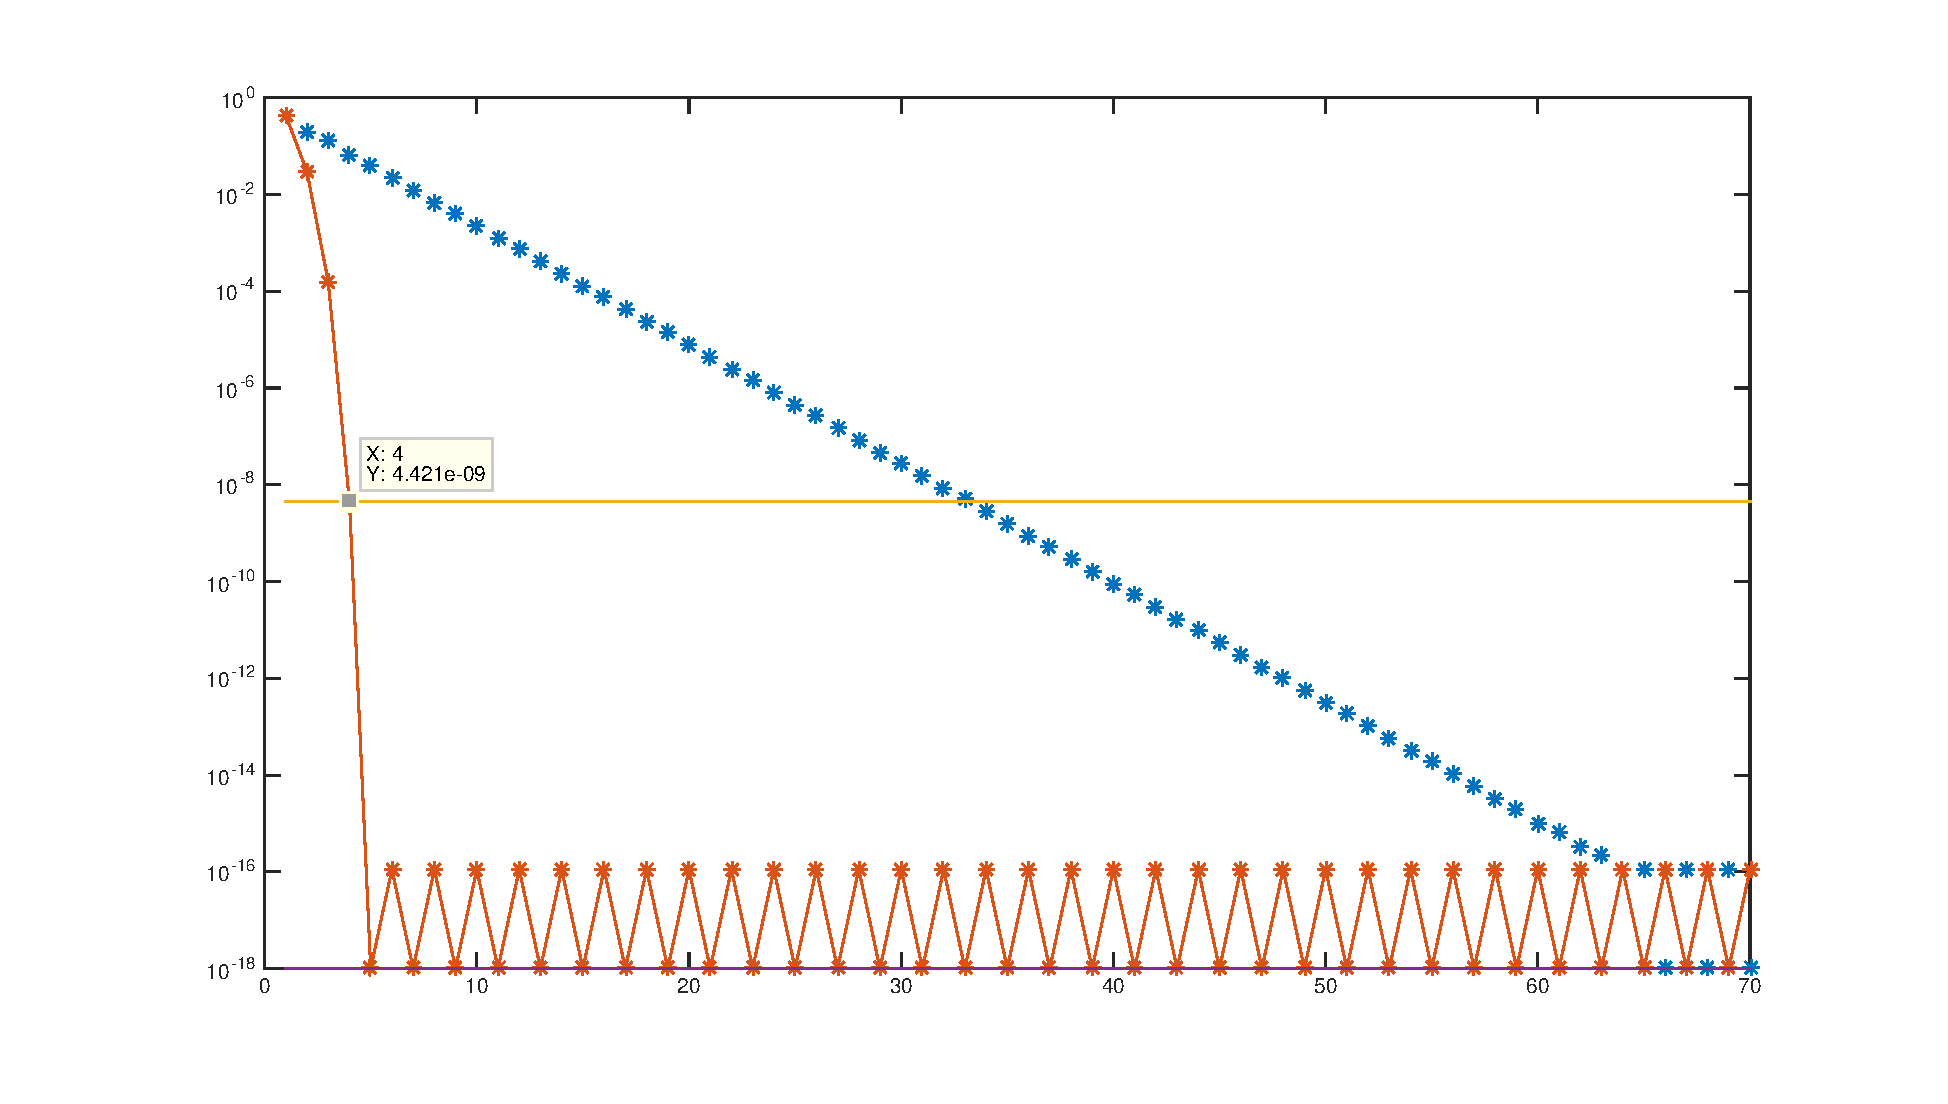
\includegraphics[width=5.5in]{1.eps}}

取初始值为1,不动点迭代要迭代65次左右才能达到Newton-Raphson迭代4次的迭代精度,迭代33次才能达到牛顿迭代3次的迭代精度。

由于牛顿迭代是二次收敛,不动点迭代是线性收敛,所以牛顿迭代法的迭代速度要快很多。


%第二题

\item 证明范数的等价关系:对于\(n\)维向量 \( \bm{x}\),当\(1 \leq p \leq q\)时有

\[
\| \bm{x} \|_{l_q} \leq \| \bm{x} \|_{l_p} \leq n^{ \frac{1}{p} - \frac{1}{q}} \| \bm{x} \|_{l_q}
\]

\begin{proof}

用数学归纳法证明


先证明\( \| \bm{x} \|_{l_q} \leq \| \bm{x} \|_{l_p} \),\(n=1\)时显然成立。再假设\(n \leq k-1\)时,依然成立,那就有

\begin{eqnarray*}
\|\bm{x}\|_{l_p} &=& (\sum_{i=1}^k x_i^p)^{\frac{1}{p}} =(\sum_{i=1}^{k-1} x_i^p+x^p_k)^{\frac{1}{p}} \nonumber \\
& \geq& ((\sum_{i=1}^{k-1} x_i^q)^{ \frac{p}{q} } + x_k^p)^{\frac{1}{p}} \nonumber \\
& \geq & ((\sum_{i=1}^{k-1} x_i^q)^{ \frac{q}{q} } +x_k^q)^{\frac{1}{q}} \nonumber \\
& =& \|\bm{x}\|_{l_q}
\end{eqnarray*}



由Jensen不等式知,当\(1 \leq p \leq q\)时
\[
(\sum^n_{i=1} \frac{|x_i|^p}{n} )^{\frac{1}{p}}\leq (\sum^n_{i=1} \frac{|x_i|^q}{n} )^{\frac{1}{q}}
\]

则
\begin{eqnarray*}
n^{-\frac{1}{p}} (\sum^n_{i=1} |x_i|^p) & \leq & n^{-\frac{1}{q}} (\sum^n_{i=1} |x_i|^q) \\
n^{-\frac{1}{p}} \| \bm{x}\|_{l_p} & \leq & n^{-\frac{1}{q}} \| \bm{x}\|_{l_q} \\
\| \bm{x} \|_{l_p} & \leq & n^{\frac{1}{p}-\frac{1}{q}} \| \bm{x}\|_{l_q} 
\end{eqnarray*}

\end{proof}
\end{enumerate}
\end{document}
